\documentclass[a4paper,10pt]{article}
\usepackage[utf8]{inputenc}

\usepackage{tikz}

%opening
\title{}
\author{}

\begin{document}


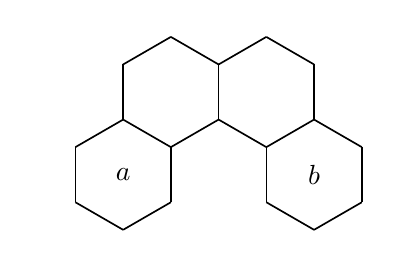
\begin{tikzpicture}[scale=0.7]
\tikzstyle{external coordinate} = []
\tikzstyle{internal coordinate} = []
\tikzstyle{border coordinate} = []
\tikzstyle{internal hexagon} = []
\tikzstyle{hexalabel}=[]
\tikzstyle{external hexagon} = []
\tikzstyle{internal vertex} = []
\tikzstyle{border vertex} = []
\tikzstyle{border edge} = [draw, color=black, semithick]
\tikzstyle{internal edge} = [draw, color=black, semithick]
\tikzstyle{external edge} = [draw, color=green]
\coordinate[external coordinate] (c_1) at (0.00000, 0.00000);
\coordinate[external coordinate] (c_2) at (0.86603, 0.50000);
\coordinate[border coordinate] (c_3) at (1.73205, 0.00000);
\coordinate[border coordinate] (c_4) at (1.73205, -1.00000);
\coordinate[border coordinate] (c_5) at (0.86603, -1.50000);
\coordinate[external coordinate] (c_6) at (0.00000, -1.00000);
\coordinate[border coordinate] (c_7) at (2.59808, 0.50000);
\coordinate[border coordinate] (c_8) at (3.46410, 0.00000);
\coordinate[border coordinate] (c_9) at (3.46410, -1.00000);
\coordinate[border coordinate] (c_10) at (2.59808, -1.50000);
\coordinate[border coordinate] (c_11) at (4.33013, 0.50000);
\coordinate[border coordinate] (c_12) at (5.19615, 0.00000);
\coordinate[border coordinate] (c_13) at (5.19615, -1.00000);
\coordinate[border coordinate] (c_14) at (4.33013, -1.50000);
\coordinate[border coordinate] (c_15) at (2.59808, -2.50000);
\coordinate[border coordinate] (c_16) at (1.73205, -3.00000);
\coordinate[border coordinate] (c_17) at (0.86603, -2.50000);
\coordinate[border coordinate] (c_18) at (4.33013, -2.50000);
\coordinate[external coordinate] (c_19) at (3.46410, -3.00000);
\coordinate[border coordinate] (c_20) at (6.06218, -1.50000);
\coordinate[border coordinate] (c_21) at (6.06218, -2.50000);
\coordinate[border coordinate] (c_22) at (5.19615, -3.00000);
\path[external hexagon] (c_1) -- (c_2) -- (c_3) -- (c_4) -- (c_5) -- (c_6) -- cycle;
%\node[hexalabel] at (0.86603, -0.50000) {$H_1$};
\path[internal hexagon] (c_3) -- (c_7) -- (c_8) -- (c_9) -- (c_10) -- (c_4) -- cycle;
%\node[hexalabel] at (2.59808, -0.50000) {$H_2$};
\path[internal hexagon] (c_8) -- (c_11) -- (c_12) -- (c_13) -- (c_14) -- (c_9) -- cycle;
%\node[hexalabel] at (4.33013, -0.50000) {$H_3$};
\path[internal hexagon] (c_5) -- (c_4) -- (c_10) -- (c_15) -- (c_16) -- (c_17) -- cycle;
\node[hexalabel] at (1.73205, -2.00000) {$a$};
\path[external hexagon] (c_10) -- (c_9) -- (c_14) -- (c_18) -- (c_19) -- (c_15) -- cycle;
%\node[hexalabel] at (3.46410, -2.00000) {$H_5$};
\path[internal hexagon] (c_14) -- (c_13) -- (c_20) -- (c_21) -- (c_22) -- (c_18) -- cycle;
\node[hexalabel] at (5.19615, -2.00000) {$b$};
\path[border edge] (c_3) -- (c_4);
\path[border edge] (c_4) -- (c_5);
\path[border edge] (c_3) -- (c_7);
\path[border edge] (c_7) -- (c_8);
\path[internal edge] (c_8) -- (c_9);
\path[border edge] (c_9) -- (c_10);
\path[internal edge] (c_10) -- (c_4);
\path[border edge] (c_8) -- (c_11);
\path[border edge] (c_11) -- (c_12);
\path[border edge] (c_12) -- (c_13);
\path[internal edge] (c_13) -- (c_14);
\path[border edge] (c_14) -- (c_9);
\path[border edge] (c_10) -- (c_15);
\path[border edge] (c_15) -- (c_16);
\path[border edge] (c_16) -- (c_17);
\path[border edge] (c_17) -- (c_5);
\path[border edge] (c_14) -- (c_18);
\path[border edge] (c_13) -- (c_20);
\path[border edge] (c_20) -- (c_21);
\path[border edge] (c_21) -- (c_22);
\path[border edge] (c_22) -- (c_18);
\node[border vertex] (v_3) at (c_3) {};
\node[border vertex] (v_4) at (c_4) {};
\node[border vertex] (v_5) at (c_5) {};
\node[border vertex] (v_7) at (c_7) {};
\node[border vertex] (v_8) at (c_8) {};
\node[border vertex] (v_9) at (c_9) {};
\node[border vertex] (v_10) at (c_10) {};
\node[border vertex] (v_11) at (c_11) {};
\node[border vertex] (v_12) at (c_12) {};
\node[border vertex] (v_13) at (c_13) {};
\node[border vertex] (v_14) at (c_14) {};
\node[border vertex] (v_15) at (c_15) {};
\node[border vertex] (v_16) at (c_16) {};
\node[border vertex] (v_17) at (c_17) {};
\node[border vertex] (v_18) at (c_18) {};
\node[border vertex] (v_20) at (c_20) {};
\node[border vertex] (v_21) at (c_21) {};
\node[border vertex] (v_22) at (c_22) {};
\end{tikzpicture}

\end{document}
